\documentclass[11pt]{article}

% Language setting
\usepackage[turkish]{babel}
\usepackage{pythonhighlight}

\usepackage[a4paper,top=2cm,bottom=2cm,left=2cm,right=2cm,marginparwidth=2cm]{geometry}

% Useful packages
\usepackage{amsmath}
\usepackage{graphicx}
\usepackage[colorlinks=true, allcolors=blue]{hyperref}
\usepackage{verbatim}
\usepackage{fancyhdr} % for header and footer
\usepackage{titlesec}
\usepackage{parskip}

\setlength{\parindent}{0pt}

\titleformat{\subsection}[runin]{\bfseries}{\thesubsection}{1em}{}

\pagestyle{fancy} % activate the custom header/footer

% define the header/footer contents
\lhead{\small{23BLM-4014 Yapay Sinir Ağları Ara Sınav Soru ve Cevap Kağıdı}}
\rhead{\small{Dr. Ulya Bayram}}
\lfoot{}
\rfoot{}

% remove header/footer on first page
\fancypagestyle{firstpage}{
  \lhead{}
  \rhead{}
  \lfoot{}
  \rfoot{\thepage}
}
 

\title{Çanakkale Onsekiz Mart Üniversitesi, Mühendislik Fakültesi, Bilgisayar Mühendisliği Akademik Dönem 2022-2023\\
Ders: BLM-4014 Yapay Sinir Ağları/Bahar Dönemi\\ 
ARA SINAV SORU VE CEVAP KAĞIDI\\
Dersi Veren Öğretim Elemanı: Dr. Öğretim Üyesi Ulya Bayram}
\author{%
\begin{minipage}{\textwidth}
\raggedright
Öğrenci Adı Soyadı: Hasan Asker Kılınç\\ % Adınızı soyadınızı ve öğrenci numaranızı noktaların yerine yazın
Öğrenci No: 210401002
\end{minipage}%
}

\date{14 Nisan 2023}

\begin{document}
\maketitle

\vspace{-.5in}
\section*{Açıklamalar:}
\begin{itemize}
    \item Vizeyi çözüp, üzerinde aynı sorular, sizin cevaplar ve sonuçlar olan versiyonunu bu formatta PDF olarak, Teams üzerinden açtığım assignment kısmına yüklemeniz gerekiyor. Bu bahsi geçen PDF'i oluşturmak için LaTeX kullandıysanız, tex dosyasının da yer aldığı Github linkini de ödevin en başına (aşağı url olarak) eklerseniz bonus 5 Puan! (Tavsiye: Overleaf)
    \item Çözümlerde ya da çözümlerin kontrolünü yapmada internetten faydalanmak, ChatGPT gibi servisleri kullanmak serbest. Fakat, herkesin çözümü kendi emeğinden oluşmak zorunda. Çözümlerinizi, cevaplarınızı aşağıda belirttiğim tarih ve saate kadar kimseyle paylaşmayınız. 
    \item Kopyayı önlemek için Github repository'lerinizin hiçbirini \textbf{14 Nisan 2023, saat 15:00'a kadar halka açık (public) yapmayınız!} (Assignment son yükleme saati 13:00 ama internet bağlantısı sorunları olabilir diye en fazla ekstra 2 saat daha vaktiniz var. \textbf{Fakat 13:00 - 15:00 arası yüklemelerden -5 puan!}
    \item Ek puan almak için sağlayacağınız tüm Github repository'lerini \textbf{en geç 15 Nisan 2023 15:00'da halka açık (public) yapmış olun linklerden puan alabilmek için!}
    \item \textbf{14 Nisan 2023, saat 15:00'dan sonra gönderilen vizeler değerlendirilmeye alınmayacak, vize notu olarak 0 (sıfır) verilecektir!} Son anda internet bağlantısı gibi sebeplerden sıfır almayı önlemek için assignment kısmından ara ara çözümlerinizi yükleyebilirsiniz yedekleme için. Verilen son tarih/saatte (14 Nisan 2023, saat 15:00) sistemdeki en son yüklü PDF geçerli olacak.
    \item Çözümlerin ve kodların size ait ve özgün olup olmadığını kontrol eden bir algoritma kullanılacaktır. Kopya çektiği belirlenen vizeler otomatikman 0 (sıfır) alacaktır. Bu nedenle çözümlerinizi ve kodlarınızı yukarıda sağladığım gün ve saatlere kadar kimseyle paylaşmayınız.
    \item Bu vizeden alınabilecek en yüksek not 100'dür. Toplam aldığınız puan 100'ü geçerse, aldığınız not 100'e sabitlenecektir.
    \item LaTeX kullanarak PDF oluşturanlar öz geçmişlerine LaTeX bildiklerini de eklemeyi unutmasınlar :)
    \item Bu vizedeki soruların çözümleri ve tex dosyası için istediğiniz kadar sayıda Github repository'si oluşturabilirsiniz. Sadece yukarıda belirttiğim tarihlerde (14 Nisan 2023 saat 15:00 ile 15 Nisan 2023 saat 15:00 arasında) public yapmayı/halka açmayı ve Github profilinizi de öz geçmişinize eklemeyi unutmayın :)
    \item Bilgisayarınıza hiçbir program kurmadan, Overleaf, Google Colab, Kaggle gibi ortamlar üzerinden bu vizeyi tamamlamanız mümkün. İyi çalışmalar!!
\end{itemize}

(Ekstra 5 puan) \url{OdevinTexDosyasınınGithubLinkiniburayakoyun.com}

\newpage
\section{(Toplam 10 Puan) Hopfield Networks:}

\subsection{(2 Puan)} \textbf{ChatGPT’ye size Hopfield Network’ler ile ilgili detaylı bilgi vermesini isteyin. Sorduğunuz soruyu, ChatGPT'nin çıkartığı cevabı aşağı koyun. Bu cevapta anlamadığınız terimleri de ChatGPT’ye sorup, sorduğunuz soruları ve ChatGPT’nin verdiği cevapları da sırayla aşağı koyun.}

\textbf{Hopfield Network nedir? Detaylı bilgi verebilir misin?}
Hopfield ağı, bir tür geri beslemeli yapay sinir ağıdır. İlk olarak John Hopfield tarafından 1982 yılında tanıtılmıştır. Hopfield ağları, bir dizi giriş vektörüne dayalı olarak öğrenme ve hafıza görevleri gerçekleştirebilir.

Hopfield ağları, asenkronik olarak güncellenen ve her biri birbirine tamamen bağlı olan bir dizi nöron kullanır. Nöronlar iki durumda olabilir: +1 veya -1. Ağın her bir nöronu, diğer nöronların durumlarından etkilenen bir ağırlık vektörüne sahiptir. Bu ağırlık vektörü, nöronlar arasındaki bağlantıların gücünü temsil eder.

Hopfield ağları, öğrenme işlemi sırasında, bir giriş vektörünün bir dizi örneği kullanılarak eğitilir. Bu eğitim işlemi, ağın bağlantı ağırlıklarının hesaplanmasını ve depolanmasını içerir. Depolanan bağlantı ağırlıkları, ağın daha sonra tanıdığı veya hatırlayabileceği örüntüleri temsil eder.

Ağın tanıma işlemi, bir giriş vektörünün ağa sunulması ve ağın depoladığı örüntülerle karşılaştırılmasıyla gerçekleşir. Ağ, giriş vektörünü depoladığı örüntüye en yakın olan örüntüye yakınsar ve çıkış olarak bu örüntüyü verir.

Hopfield ağları, özellikle hatırlama ve tanıma problemlerinde kullanılır. Bunlar, örneğin yüz tanıma, yazı tanıma veya nesne tanıma gibi alanlarda kullanılabilir. Hopfield ağları, doğrusal olarak ayrılabilen olmayan problemleri çözmek için de kullanılabilirler.

\textbf{"bir giriş vektörünün bir dizi örneği kullanılarak eğitilir" bu tarz bir işlem nasıl yapılır? Basitçe kod üzerinden tanımla}.
Hopfield ağının öğrenme işlemi, verilen bir dizi örnek vektörü üzerinden yapılır. Bu örnek vektörleri aynı boyutta olmalıdır ve her bir elemanı +1 veya -1 olmalıdır.

Aşağıdaki Python kodu, iki örnek vektörü kullanarak bir Hopfield ağı öğrenme işlemini gösterir:
\begin{python}
    
import numpy as np

# iki örnek vektörümüz
pattern1 = np.array([1, -1, 1, -1])
pattern2 = np.array([-1, 1, -1, 1])

# örnek vektörlerimizi birleştiriyoruz
patterns = np.array([pattern1, pattern2])

# ağın ağırlık matrisini başlatıyoruz
weights = np.zeros((patterns.shape[1], patterns.shape[1]))

# ağırlık matrisini hesaplıyoruz
for pattern in patterns:
    weights += np.outer(pattern, pattern)

# diagonal elemanları sıfırlıyoruz
np.fill_diagonal(weights, 0)

# ağın öğrenme işlemi tamamlandı
\end{python}
Bu kodda, öncelikle iki örnek vektör tanımlanır. Sonra bu iki örnek vektörü birleştirilir ve bir ağırlık matrisi başlatılır. Ardından, örnek vektörlerinden yararlanarak ağırlık matrisi hesaplanır. Son olarak, ağırlık matrisinin diagonal elemanları sıfırlanır.

Bu örnek kodda, iki örnek vektörü kullanarak bir Hopfield ağı öğrenme işlemi gösterilmiştir. Daha fazla örnek vektörü kullanarak ağırlık matrisinin daha doğru hesaplanması mümkündür.

\subsection{(8 Puan)} \textbf{ChatGPT’nin açıklamalarından ne anladığınızı buraya kendi kelimelerinizle özetleyin. Örneğin ``Hopfield Network nedir? Ne işe yarar? Neden bilmemiz gerekir bunu? Gerçek hayatta kullanılıyor mu?'' gibi. Anlamadığınız kısımlar varsa ve ChatGPT’nin açıklamaları yeterli gelmezse internet dahil farklı kaynaklardan araştırıp, bilgilerin doğruluğunu sorgulamakta serbestsiniz. Konuyu doğru anlayıp anlamamanız puana etki edecektir. Kullandığınız kaynakları da belirtin!}

{Hopfield ağları, basit bir yapısı olan geri beslemeli sinir ağı modelleridir. Temel amacı, örnekleri hatırlama ve geri çağırma işlemidir. Her bir düğümün sadece "etkin veya etkisiz" olarak iki durumda olabilmesi, ağırlıkların hesaplanmasını kolaylaştırır. Özellikle küçük boyutlu problemler için tercih edilen yapay zeka ve sinir ağı modelleri arasındadır. Örnek olarak, hafıza ve veri sıkıştırma işlemlerinde kullanılabilirler. 

Hopfield ağını çalıştırmanın temel yolu, nöronları rastgele ve bağlı nöronları ağırlıklarıyla birlikte dikkate alarak tekrarlamaktır. Kısaca özetlemek gerekirse, hopfield ağ modeli, her biri birbirine bağlı sinir hücrelerinden oluşan bir kümedir. Girdi ve çıktı kümeleri arasında fark yoktur.

\begin{enumerate}
\item Şifreleme işlemlerinde
\item Karakter-Desen Eşleştirmede
\item Bozuk Şekillerin Yeniden Oluşturulmasında
\item El Yazı Tanımlama Sistemlerinde
\end{enumerate}

}

\section{(Toplam 10 Puan) Boltzman Machine:}

\subsection{(2 Puan)} \textbf{ChatGPT’ye size Boltzman Machine ilgili detaylı bilgi vermesini isteyin. Sorduğunuz soruyu, ChatGPT'nin çıkartığı cevabı aşağı koyun. Bu cevapta anlamadığınız terimleri de ChatGPT’ye sorup, sorduğunuz soruları ve ChatGPT’nin verdiği cevapları da sırayla aşağı koyun.}

\textbf{Boltzman machine nedir? Detaylı bilgi verebilir misin?}

Boltzmann Machine (BM), yapay sinir ağı modellerinden biridir. Hava moleküllerinin davranışını modelleyen fiziksel bir sistem olan Boltzmann makineleri tarafından ilham alınarak geliştirilmiştir. BM, belirli bir veri kümesindeki örüntüleri tanımlamak ve öğrenmek için kullanılır.

BM'nin temel yapısı, girdi ve çıktı katmanları arasında bir veya daha fazla gizli katman içeren bir ölçümlü sinir ağıdır. BM, ağırlıkları ayarlamak için bir öğrenme algoritması kullanır. Öğrenme sırasında, ağ verilen veri kümesine uyarlanır ve ardından yeni verileri sınıflandırır.

BM, unsupervised learning (denetimsiz öğrenme) yöntemlerinden biridir. Veri kümesindeki örüntüleri tanımlamak ve kategorize etmek için kullanılır. BM, öğrenme sırasında stokastik gradient iniş algoritmasını kullanır ve ağırlıkları rastgele başlatır. Daha sonra, ağ öğrenme sırasında öznitelikleri öğrenir ve ağırlıkları ayarlar.

BM, özellikle görüntü işleme, doğal dil işleme ve ses tanıma gibi alanlarda kullanılmaktadır. BM, bu alanlarda yüksek doğruluk oranları elde etmek için kullanılan en gelişmiş yapay sinir ağı modellerinden biridir. BM'nin bir dezavantajı, öğrenme sırasında uzun süreli hafızasının olmamasıdır.

Sonuç olarak, Boltzmann Machine, belirli bir veri kümesindeki örüntüleri tanımlamak ve öğrenmek için kullanılan bir yapay sinir ağı modelidir. Özellikle görüntü işleme, doğal dil işleme ve ses tanıma gibi alanlarda yüksek doğruluk oranları elde etmek için kullanılmaktadır.

 \textbf{unsupervised learning (denetimsiz öğrenme) nedir? Basit bir şeklide anlatır mısın?}
Denetimsiz öğrenme, makine öğrenimi alanında bir öğrenme yöntemidir ve eğitim verilerinin etiketlenmemesi veya kategorize edilmemesi durumunda kullanılır. Bu yöntemde, algoritma, veriler arasındaki doğal yapıları öğrenir ve bu yapıları kullanarak verileri gruplandırır veya düzenler.

Denetimsiz öğrenme, verilerin özelliklerini, kalıplarını ve yapılarını keşfetmek için kullanılır. Verilerin gizli yapısını belirlemek ve veriler arasındaki ilişkileri anlamak için farklı yöntemler kullanılır. Kümelenme (clustering), boyut azaltma (dimensionality reduction), ilişki kurma (association) ve anomalileri tespit etme (anomaly detection) gibi denetimsiz öğrenme teknikleri, bu alanda sıklıkla kullanılan yöntemlerdir.

Denetimsiz öğrenmenin birçok uygulaması vardır, örneğin müşteri segmentasyonu, sosyal medya analizi, tıbbi görüntü işleme, dil işleme, arama motorları, robotik ve otomatik sürüş gibi alanlarda kullanılır. Bu uygulamaların çoğu, verilerin anlamlı bir şekilde gruplandırılması veya yapılandırılması gerektiği durumlarda kullanılır.

\textbf{boltzman machine neden öğrenme sırasında uzun süreli hafızasının olmadığını açıkla}
Boltzmann makineleri, her bir veri örneği için ayrı bir model oluşturmak yerine bir tane model kullanarak tüm veri örneklerinin ortak özelliklerini öğrenmeye çalışır. Bu nedenle, öğrenme sırasında Boltzmann makineleri sadece o anda gözlemledikleri verilere dayanarak öğrenirler ve her bir örnek üzerinde ayrı ayrı işlem yapmazlar.

Bunun sonucu olarak, Boltzmann makineleri öğrenme sırasında sadece kısa süreli bellek (short-term memory) kullanırlar. Yani, öğrenme sürecinde öğrenilen bilgiler, öğrenme işlemi tamamlandıktan sonra unutulabilir. Bu nedenle, Boltzmann makineleri genellikle öğrenme sonrası kullanım için tercih edilirler.

Uzun süreli bellek (long-term memory) özellikle birçok yinelemeli öğrenme (iterative learning) işlemi gerektiren derin öğrenme modellerinde kullanılır. Bu modeller, ağın önceki aşamalarında öğrenilen bilgileri, sonraki aşamalarda kullanarak daha iyi sonuçlar elde ederler. Bu süreçte, öğrenilen bilgiler, ağın ağırlık matrislerinde depolanır ve her bir iterasyonda güncellenir.



\subsection{(8 Puan)} \textbf{ChatGPT’nin açıklamalarından ne anladığınızı buraya kendi kelimelerinizle özetleyin. Örneğin ``Boltzman Machine nedir? Ne işe yarar? Neden bilmemiz gerekir bunu? Gerçek hayatta kullanılıyor mu?'' gibi. Anlamadığınız kısımlar varsa ve ChatGPT’nin açıklamaları yeterli gelmezse internet dahil farklı kaynaklardan araştırıp, bilgilerin doğruluğunu sorgulamakta serbestsiniz. Konuyu doğru anlayıp anlamamanız puana etki edecektir. Kullandığınız kaynakları da belirtin!}

Sınıflandırma, regrasyon ve özellik öğrenimi işlemlerini yapan boltzman makinesi giriş veri seti üzerinde olasılıksal dağılımları öğrenebilen bir sinir ağıdır. Bir Boltzmann makinesi, stokastik tekrarlayan sinir ağı tipidir. Boltzmann makineleri Hopfield ağlarının stokastik, üretken karşılığı olarak görülebilir. Bunlar, iç temsilleri öğrenebilen ilk sinir ağlarındandır ve zor kombinatoryal problemleri temsil edip çözebilirler. Sınırsız bağlanabilirliği olan Boltzmann makineleri, makine öğrenmesi veya çıkarımında pratik sorunlar için yararlı değildir, ancak eğer bağlantı düzgün bir şekilde kısıtlıysa, öğrenme pratik problemler için faydalı olacak kadar verimli hale getirilebilir.

Boltzmann Machine hakkında bazı önemli noktalar :
\begin{enumerate}
\item Tekrarlayan yapı kullanırlar.
\item 1 veya 0 olmak üzere iki olası durumdan birine sahip olan stokastik nöronlardan oluşurlar.
\item Buradaki nöronlardan bazıları uyarlanabilir serbest durum
  ve bazıları donmuş durumda sıkıştırılır.
  \item Ayrık Hopfield ağında benzetilmiş tavlama uygularsak, Boltzmann Makinesi olur.
\end{enumerate}

\textit{\url{https://en.wikipedia.org/wiki/Boltzmann_machine}
}


\section{(Toplam 10 Puan) Markov Assumption ve Markov Chain:}

\subsection{(2 Puan)} \textbf{ChatGPT’ye size Markov assumption ve Markov Chain ilgili detaylı bilgi vermesini isteyin. Sorduğunuz soruyu, ChatGPT'nin çıkartığı cevabı aşağı koyun. Bu cevapta anlamadığınız terimleri de ChatGPT’ye sorup, sorduğunuz soruları ve ChatGPT’nin verdiği cevapları da sırayla aşağı koyun.}

\textbf{Markov Assumption ve Markov Chain nedir? Nerelerde kullanılır, ne için kullanılır, kullanırsak bize ne gibi avantajlar sağlar. Olmasaydı ne olurdu?}
Markov Assumption (Markov varsayımı), gelecekteki durumların sadece mevcut durumla ilgili olduğu ve geçmiş durumlarla bağlantısının olmadığı varsayımıdır. Bu varsayım, birçok makine öğrenmesi ve istatistiksel modelleme tekniklerinde kullanılır.

Markov Chain (Markov zinciri), Markov Assumption kullanılarak tanımlanmış bir olasılık sürecidir. Bir Markov zinciri, bir dizi durumdan oluşur ve her bir durum, yalnızca mevcut duruma bağlıdır ve geçmiş durumlarla ilgisi yoktur. Markov zinciri, gelecekteki durumların tahmin edilmesi ve olasılıkların hesaplanması için kullanılır.

Markov Assumption ve Markov Chain birçok alanda kullanılır. Örneğin, doğal dil işlemede, bir kelimenin anlamını tahmin etmek için önceki kelimeler yerine yalnızca en son kelimeyi kullanabilirsiniz. Ayrıca, ekonometride, ekonomik değişkenler arasındaki ilişkileri modellerken de kullanılır.

Markov Assumption ve Markov Chain kullanmanın avantajlarından bazıları şunlardır:
\begin{enumerate}
    \item Geçmiş verilerin depolanmasına ihtiyaç yoktur, bu nedenle depolama maliyetleri düşüktür.
    \item Tahminler ve olasılıklar hızlı bir şekilde hesaplanabilir.

\item Bu varsayım, daha büyük ve daha karmaşık modellerin oluşturulmasını kolaylaştırır.

\end{enumerate}
 Eğer Markov Assumption ve Markov Chain kullanılmasaydı, daha önceki durumlar göz önüne alınmadığından, gelecekteki durumlar daha az doğru bir şekilde tahmin edilebilirdi ve olasılıkların hesaplanması daha zor hale gelirdi.



\subsection{(8 Puan)} \textbf{ChatGPT’nin açıklamalarından ne anladığınızı buraya kendi kelimelerinizle özetleyin. Örneğin ``Markov assumption ve Markov Chain nedir? Ne işe yarar? Neden bilmemiz gerekir bunu? Gerçek hayatta kullanılıyor mu?'' gibi. Anlamadığınız kısımlar varsa ve ChatGPT’nin açıklamaları yeterli gelmezse internet dahil farklı kaynaklardan araştırıp, bilgilerin doğruluğunu sorgulamakta serbestsiniz. Konuyu doğru anlayıp anlamamanız puana etki edecektir. Kullandığınız kaynakları da belirtin!}

"Bir Markov zinciri veya Markov süreci, her olayın olasılığının yalnızca önceki olayda elde edilen duruma bağlı olduğu olası olaylar dizisini tanımlayan stokastik (rastlantısal) bir modeldir. Zincirin ayrık (discrete) zaman adımlarında durumu hareket ettirdiği, sonsuz (countably infinite) bir dizi, ayrık zamanlı bir Markov zinciri (DTMC) verir. Sürekli zamanlı bir süreç, sürekli zamanlı Markov zinciri (CTMC) olarak adlandırılır. Adını Rus matematikçi Andrey Markov'dan almıştır.

Markov zincirleri, gerçek dünya süreçlerinin istatistiksel modelleri olarak birçok uygulamaya sahiptir, örneğin motorlu taşıtlardaki hız kontrol sistemlerini, bir havaalanına gelen müşteri kuyruklarını veya hatlarını, döviz kurlarını ve döviz kurlarını ve hayvan popülasyonu dinamikleri gibi konuları incelemek için kullanılabilir.

Markov süreçleri, karmaşık olasılık dağılımlarından örneklemeyi simüle etmek için kullanılan ve Bayes istatistikleri, termodinamik, istatistiksel mekanik, fizik, kimya, ekonomi, finans, sinyal alanlarında uygulama bulan Markov zinciri Monte Carlo olarak bilinen genel stokastik simülasyon yöntemlerinin  ve işleme, bilgi teorisi ve konuşma işlemenin temelidir.

\url{https://tr.wikipedia.org/wiki/Markov_zinciri#:~:text=Matematikte%2C%20Markov%20Zinciri%20(Andrey%20Markov,durumlardan%20ba%C4%9F%C4%B1ms%C4%B1z%20olmas%C4%B1%20anlam%C4%B1na%20gelir.}

\section{(Toplam 20 Puan) Feed Forward:}
 
\begin{itemize}
    \item Forward propagation için, input olarak şu X matrisini verin (tensöre çevirmeyi unutmayın):\\
    $X = \begin{bmatrix}
        1 & 2 & 3\\
        4 & 5 & 6
        \end{bmatrix}$
    Satırlar veriler (sample'lar), kolonlar öznitelikler (feature'lar).
    \item Bir adet hidden layer olsun ve içinde tanh aktivasyon fonksiyonu olsun
    \item Hidden layer'da 50 nöron olsun
    \item Bir adet output layer olsun, tek nöronu olsun ve içinde sigmoid aktivasyon fonksiyonu olsun
\end{itemize}

Tanh fonksiyonu:\\
$f(x) = \frac{exp(x) - exp(-x)}{exp(x) + exp(-x)}$
\vspace{.2in}

Sigmoid fonksiyonu:\\
$f(x) = \frac{1}{1 + exp(-x)}$

\vspace{.2in}
 \textbf{Pytorch kütüphanesi ile, ama kütüphanenin hazır aktivasyon fonksiyonlarını kullanmadan, formülünü verdiğim iki aktivasyon fonksiyonunun kodunu ikinci haftada yaptığımız gibi kendiniz yazarak bu yapay sinir ağını oluşturun ve aşağıdaki üç soruya cevap verin.}
 
\subsection{(10 Puan)} \textbf{Yukarıdaki yapay sinir ağını çalıştırmadan önce pytorch için Seed değerini 1 olarak set edin, kodu aşağıdaki kod bloğuna ve altına da sonucu yapıştırın:}

% Latex'de kod koyabilirsiniz python formatında. Aşağıdaki örnekleri silip içine kendi kodunuzu koyun
\begin{python}
import torch
import torch.nn as nn
import numpy as np

torch.manual_seed(1)

x = [[1,2,3],[4,5,6]]
tensor = torch.tensor(x, dtype=torch.float32)
tensor=tensor.reshape(1,6)

def sigmoid_activation(x):
  return 1 / (1 + torch.exp(-x))

def tanh_activation(x):
    return (torch.exp(x) - torch.exp(-x)) / (torch.exp(x) + torch.exp(-x)) 

class MLP(nn.Module):
    def __init__(self, num_of_input_features, num_of_hidden_neurons, num_of_output_neurons):
        super(MLP, self).__init__()
        self.hidden_layer = nn.Linear(num_of_input_features, num_of_hidden_neurons)
        self.output_layer = nn.Linear(num_of_hidden_neurons, num_of_output_neurons)

        nn.init.normal_(self.hidden_layer.weight)
        nn.init.normal_(self.hidden_layer.bias)
        nn.init.normal_(self.output_layer.weight)
        nn.init.normal_(self.output_layer.bias)

    def forward(self, x):
        x = tanh_activation(self.hidden_layer(x))
        x = sigmoid_activation(self.output_layer(x))
        return x

input_shape = 6
hidden_size = 50
output_size = 1
model = MLP(input_shape, hidden_size, output_size)
y_pred = model(tensor)
print(y_pred)
\end{python}

{tensor([[0.9958]], grad_fn=<MulBackward0>)}

\subsection{(5 Puan)} \textbf{Yukarıdaki yapay sinir ağını çalıştırmadan önce Seed değerini öğrenci numaranız olarak değiştirip, kodu aşağıdaki kod bloğuna ve altına da sonucu yapıştırın:}

\begin{python}
import torch
import torch.nn as nn
import numpy as np

torch.manual_seed(210401002)

x = [[1,2,3],[4,5,6]]
tensor = torch.tensor(x, dtype=torch.float32)
tensor=tensor.reshape(1,6)

def sigmoid_activation(x):

  return 1 / (1 + torch.exp(-x))

def tanh_activation(x):
    return (torch.exp(x) - torch.exp(-x)) / (torch.exp(x) + torch.exp(-x)) 

class MLP(nn.Module):
    def __init__(self, num_of_input_features, num_of_hidden_neurons, num_of_output_neurons):
        super(MLP, self).__init__()
        self.hidden_layer = nn.Linear(num_of_input_features, num_of_hidden_neurons)
        self.output_layer = nn.Linear(num_of_hidden_neurons, num_of_output_neurons)

        nn.init.normal_(self.hidden_layer.weight)
        nn.init.normal_(self.hidden_layer.bias)
        nn.init.normal_(self.output_layer.weight)
        nn.init.normal_(self.output_layer.bias)

    def forward(self, x):
        x = tanh_activation(self.hidden_layer(x))
        x = sigmoid_activation(self.output_layer(x))
        return x

input_shape = 6
hidden_size = 50
output_size = 1
model = MLP(input_shape, hidden_size, output_size)
y_pred = model(tensor)
print(y_pred)
\end{python}
{tensor([[0.0075]], grad_fn=<MulBackward0>)}


\subsection{(5 Puan)} \textbf{Kodlarınızın ve sonuçlarınızın olduğu jupyter notebook'un Github repository'sindeki linkini aşağıdaki url kısmının içine yapıştırın. İlk sayfada belirttiğim gün ve saate kadar halka açık (public) olmasın:}
% size ait Github olmak zorunda, bu vize için ayrı bir github repository'si açıp notebook'u onun içine koyun. Kendine ait olmayıp da arkadaşının notebook'unun linkini paylaşanlar 0 alacak.

\url{https://github.com/Ask-er/artificial-neural-network-midterm/blob/main/question4.ipynb}

\section{(Toplam 40 Puan) Multilayer Perceptron (MLP):} 
\textbf{Bu bölümdeki sorularda benim vize ile beraber paylaştığım Prensesi İyileştir (Cure The Princess) Veri Seti parçaları kullanılacak. Hikaye şöyle (soruyu çözmek için hikaye kısmını okumak zorunda değilsiniz):} 

``Bir zamanlar, çok uzaklarda bir ülkede, ağır bir hastalığa yakalanmış bir prenses yaşarmış. Ülkenin kralı ve kraliçesi onu iyileştirmek için ellerinden gelen her şeyi yapmışlar, ancak denedikleri hiçbir çare işe yaramamış.

Yerel bir grup köylü, herhangi bir hastalığı iyileştirmek için gücü olduğu söylenen bir dizi sihirli malzemeden bahsederek kral ve kraliçeye yaklaşmış. Ancak, köylüler kral ile kraliçeyi, bu malzemelerin etkilerinin patlayıcı olabileceği ve son zamanlarda yaşanan kuraklıklar nedeniyle bu malzemelerden sadece birkaçının herhangi bir zamanda bulunabileceği konusunda uyarmışlar. Ayrıca, sadece deneyimli bir simyacı bu özelliklere sahip patlayıcı ve az bulunan malzemelerin belirli bir kombinasyonunun prensesi iyileştireceğini belirleyebilecekmiş.

Kral ve kraliçe kızlarını kurtarmak için umutsuzlar, bu yüzden ülkedeki en iyi simyacıyı bulmak için yola çıkmışlar. Dağları tepeleri aşmışlar ve nihayet "Yapay Sinir Ağları Uzmanı" olarak bilinen yeni bir sihirli sanatın ustası olarak ün yapmış bir simyacı bulmuşlar.

Simyacı önce köylülerin iddialarını ve her bir malzemenin alınan miktarlarını, ayrıca iyileşmeye yol açıp açmadığını incelemiş. Simyacı biliyormuş ki bu prensesi iyileştirmek için tek bir şansı varmış ve bunu doğru yapmak zorundaymış. (Original source: \url{https://www.kaggle.com/datasets/unmoved/cure-the-princess})

(Buradan itibaren ChatGPT ve Dr. Ulya Bayram'a ait hikayenin devamı)

Simyacı, büyülü bileşenlerin farklı kombinasyonlarını analiz etmek ve denemek için günler harcamış. Sonunda birkaç denemenin ardından prensesi iyileştirecek çeşitli karışım kombinasyonları bulmuş ve bunları bir veri setinde toplamış. Daha sonra bu veri setini eğitim, validasyon ve test setleri olarak üç parçaya ayırmış ve bunun üzerinde bir yapay sinir ağı eğiterek kendi yöntemi ile prensesi iyileştirme ihtimalini hesaplamış ve ikna olunca kral ve kraliçeye haber vermiş. Heyecanlı ve umutlu olan kral ve kraliçe, simyacının prensese hazırladığı ilacı vermesine izin vermiş ve ilaç işe yaramış ve prenses hastalığından kurtulmuş.

Kral ve kraliçe, kızlarının hayatını kurtardığı için simyacıya krallıkta kalması ve çalışmalarına devam etmesi için büyük bir araştırma bütçesi ve çok sayıda GPU'su olan bir server vermiş. İyileşen prenses de kendisini iyileştiren yöntemleri öğrenmeye merak salıp, krallıktaki üniversitenin bilgisayar mühendisliği bölümüne girmiş ve mezun olur olmaz da simyacının yanında, onun araştırma grubunda çalışmaya başlamış. Uzun yıllar birlikte krallıktaki insanlara, hayvanlara ve doğaya faydalı olacak yazılımlar geliştirmişler, ve simyacı emekli olduğunda prenses hem araştırma grubunun hem de krallığın lideri olarak hayatına devam etmiş.

Prenses, kendisini iyileştiren veri setini de, gelecekte onların izinden gidecek bilgisayar mühendisi prensler ve prensesler başkalarına faydalı olabilecek yapay sinir ağları oluşturmayı öğrensinler diye halka açmış ve sınavlarda kullanılmasını salık vermiş.''

\textbf{İki hidden layer'lı bir Multilayer Perceptron (MLP) oluşturun beşinci ve altıncı haftalarda yaptığımız gibi. Hazır aktivasyon fonksiyonlarını kullanmak serbest. İlk hidden layer'da 100, ikinci hidden layer'da 50 nöron olsun. Hidden layer'larda ReLU, output layer'da sigmoid aktivasyonu olsun.}

\textbf{Output layer'da kaç nöron olacağını veri setinden bakıp bulacaksınız. Elbette bu veriye uygun Cross Entropy loss yöntemini uygulayacaksınız. Optimizasyon için Stochastic Gradient Descent yeterli. Epoch sayınızı ve learning rate'i validasyon seti üzerinde denemeler yaparak (loss'lara overfit var mı diye bakarak) kendiniz belirleyeceksiniz. Batch size'ı 16 seçebilirsiniz.}

\subsection{(10 Puan)} \textbf{Bu MLP'nin pytorch ile yazılmış class'ının kodunu aşağı kod bloğuna yapıştırın:}

\begin{python}
class MLP(nn.Module):
    def __init__(self, input_size, hidden_size_1, hidden_size_2, output_size):
        super(MLP, self).__init__()
        self.hidden_layer1 = nn.Linear(input_size, hidden_size_1)
        self.hidden_layer2 = nn.Linear(hidden_size_1, hidden_size_2)
        self.output_layer = nn.Linear(hidden_size_2, output_size)
        self.ReLu = nn.ReLU()
        self.sigmoid = nn.Sigmoid()
    def forward(self, x):

        hidden_res1 = self.ReLu(self.hidden_layer1(x))
        hidden_res2 = self.ReLu(self.hidden_layer2(hidden_res1))
        output = self.sigmoid(self.output_layer(hidden_res2))
        return output
\end{python}

\subsection{(10 Puan)} \textbf{SEED=öğrenci numaranız set ettikten sonra altıncı haftada yazdığımız gibi training batch'lerinden eğitim loss'ları, validation batch'lerinden validasyon loss değerlerini hesaplayan kodu aşağıdaki kod bloğuna yapıştırın ve çıkan figürü de alta ekleyin.}

\begin{python}
learning_rate = 0.0001
num_epochs = 30
patience = 5

num_input_feats = len(classes) - 1
num_of_hidden_size_1, num_of_hidden_size_2 = 100, 50
num_of_output = 1

model = MLP(num_input_feats,num_of_hidden_size_1,num_of_hidden_size_2, num_of_output)

# Loss function ve optimizer
criterion = nn.BCELoss()

optimizer = torch.optim.Adam(model.parameters(), lr=learning_rate)

list_train_loss, list_val_loss = [], []
best_val_loss = None
patience_counter = 0

# Train the model
for epoch in range(num_epochs):

    # training loop
    train_loss = 0.0
    train_count = 0.0
    for inputs, labels in train_loader:
        model.train()
        # zero the parameter gradients
        optimizer.zero_grad()
        # forward + backward + optimize
        outputs = model(inputs)
        loss = criterion(outputs, labels.unsqueeze(1))
        loss.backward()
        optimizer.step()
        train_count += 1.0
        train_loss += loss.item()
     
    val_loss = 0.0
    with torch.no_grad():
        model.eval()
        for inputs, labels in validation_loader:
            outputs = model(inputs)
            loss = criterion(outputs, labels.unsqueeze(1))
            #validation_count += 1.0
            val_loss += loss.item()
  
    # calculate metrics
    train_loss /= train_count
    val_loss /= len(validation_loader)
    print("Epoch", epoch, "Training loss", train_loss,"Validation Loss :",val_loss)
    list_train_loss.append(train_loss)
    list_val_loss.append(val_loss)
    val_score = val_loss
    if best_val_loss is None:
        best_val_loss = val_score # hafızada patience boyu tutmaya başla
        torch.save(model.state_dict(), "checkpoint.pt")
    elif best_val_loss < val_score: # patience counter
        patience_counter += 1
        print("Earlystopping Patience Counter:",patience_counter)
        if patience_counter == patience:
            break
    else:
        best_val_loss = val_score
        torch.save(model.state_dict(), "checkpoint.pt") # to keep the best model
        patience_counter = 0
\end{python}

% Figure aşağıda comment içindeki kısımdaki gibi eklenir.

\begin{figure}[htbp]
  \centering
  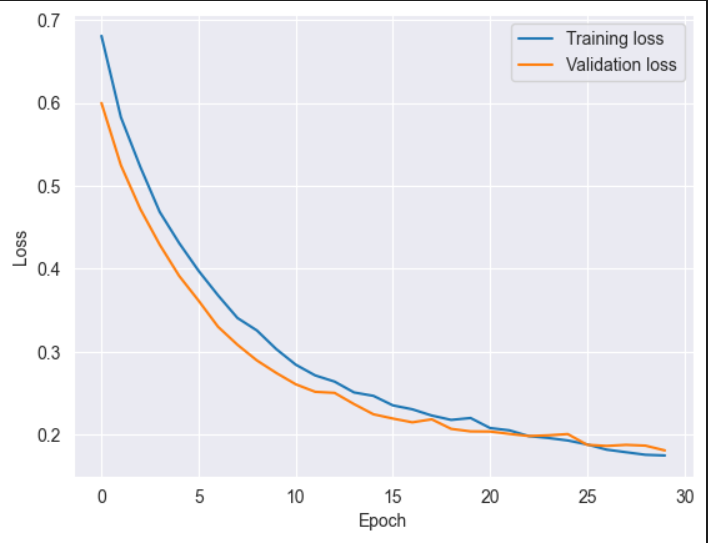
\includegraphics[width=0.8\textwidth]{./result.png}
  \caption{Result.}
  \label{RESULT}
\end{figure}


\subsection{(10 Puan)} \textbf{SEED=öğrenci numaranız set ettikten sonra altıncı haftada ödev olarak verdiğim gibi earlystopping'deki en iyi modeli kullanarak, Prensesi İyileştir test setinden accuracy, F1, precision ve recall değerlerini hesaplayan kodu yazın ve sonucu da aşağı yapıştırın. \%80'den fazla başarı bekliyorum test setinden. Daha düşükse başarı oranınız, nerede hata yaptığınızı bulmaya çalışın. \%90'dan fazla başarı almak mümkün (ben denedim).}

\begin{python}
from sklearn.metrics import f1_score,accuracy_score,classification_report,recall_score,precision_score
torch.manual_seed(210401002)

model = MLP(num_input_feats,num_of_hidden_size_1,num_of_hidden_size_2,num_of_output,)

checkpoint = torch.load("checkpoint.pt")
model.load_state_dict(checkpoint)

test_loss = 0.0
test_count = 0.0
y_true, y_pred = [], []
with torch.no_grad():
    model.eval()
    for inputs, labels in test_loader:
        outputs = model(inputs)
        loss = criterion(outputs, labels.unsqueeze(1))
        test_count += 1.0
        test_loss += loss.item()
        predicted = (outputs > 0.5).float()
        y_true.extend(labels.numpy())
        y_pred.extend(predicted.numpy().flatten())

# calculate evaluation metrics
accuracy = np.mean(np.array(y_true) == np.array(y_pred))
precision = precision_score(y_true, y_pred, average="weighted")
recall = recall_score(y_true, y_pred, average="weighted")
f1 = f1_score(y_true, y_pred, average="weighted")

print("Test loss: {:.4f}, Accuracy: {:.4f}, Precision: {:.4f}, Recall: {:.4f}, F1 score: {:.4f}".format(
    test_loss/test_count, accuracy, precision, recall, f1))
\end{python}

Test loss: 0.1818, Accuracy: 0.9339, Precision: 0.9358, Recall: 0.9339, F1 score: 0.9339

\subsection{(5 Puan)} \textbf{Tüm kodların CPU'da çalışması ne kadar sürüyor hesaplayın. Sonra to device yöntemini kullanarak modeli ve verileri GPU'ya atıp kodu bir de böyle çalıştırın ve ne kadar sürdüğünü hesaplayın. Süreleri aşağıdaki tabloya koyun. GPU için Google Colab ya da Kaggle'ı kullanabilirsiniz, iki ortam da her hafta saatlerce GPU hakkı veriyor.}

\begin{table}[ht!]
    \centering
    \caption{Buraya bir açıklama yazın}
    \begin{tabular}{c|c}
        Ortam & Süre (saniye) \\\hline
        CPU & kaç? \\
        GPU & kaç?\\
    \end{tabular}
    \label{tab:my_table}
\end{table}

\subsection{(3 Puan)} \textbf{Modelin eğitim setine overfit etmesi için elinizden geldiği kadar kodu gereken şekilde değiştirin, validasyon loss'unun açıkça yükselmeye başladığı, training ve validation loss'ları içeren figürü aşağı koyun ve overfit için yaptığınız değişiklikleri aşağı yazın. Overfit, tam bir çanak gibi olmalı ve yükselmeli. Ona göre parametrelerle oynayın.}

Cevaplar buraya

% Figür aşağı
\begin{comment}
\begin{figure}[ht!]
    \centering
    \includegraphics[width=0.75\textwidth]{mypicturehere.png}
    \caption{Buraya açıklama yazın}
    \label{fig:my_pic}
\end{figure}
\end{comment}

\subsection{(2 Puan)} \textbf{Beşinci soruya ait tüm kodların ve cevapların olduğu jupyter notebook'un Github linkini aşağıdaki url'e koyun.}

\url{https://github.com/Ask-er/artificial-neural-network-midterm/blob/main/question5.ipynb}

\section{(Toplam 10 Puan)} \textbf{Bir önceki sorudaki Prensesi İyileştir problemindeki yapay sinir ağınıza seçtiğiniz herhangi iki farklı regülarizasyon yöntemi ekleyin ve aşağıdaki soruları cevaplayın.} 

\subsection{(2 puan)} \textbf{Kodlarda regülarizasyon eklediğiniz kısımları aşağı koyun:} 

\begin{python}
kod_buraya = None
if kod_buraya:
    devam_ise_buraya = 0

print(devam_ise_buraya)
\end{python}

\subsection{(2 puan)} \textbf{Test setinden yeni accuracy, F1, precision ve recall değerlerini hesaplayıp aşağı koyun:}

Sonuçlar buraya.

\subsection{(5 puan)} \textbf{Regülarizasyon yöntemi seçimlerinizin sebeplerini ve sonuçlara etkisini yorumlayın:}

Yorumlar buraya.

\subsection{(1 puan)} \textbf{Sonucun github linkini  aşağıya koyun:}

\url{www.benimgithublinkim2.com}

\end{document}